\documentclass[a4paper,12pt]{article} % article, report, book
\usepackage{ifthen}

\usepackage{fontspec}

\setmainfont[Ligatures={Common,TeX}]{TeXGyreTermes-Regular}
\setsansfont[Ligatures={Common,TeX}]{Droid Sans}
\setmonofont{CMU Typewriter Text}
\defaultfontfeatures{Mapping=tex-text,Scale=MatchLowercase}

\usepackage{luatexja-fontspec}
\setmainjfont[BoldFont={SimHei},ItalicFont={KaiTi}]{SimSun}
\setsansjfont{KaiTi}
\defaultjfontfeatures{JFM=kaiming}
\newjfontfamily\HEI{SimSun}
\newjfontfamily\KAI{SimSun}
\newjfontfamily\FANGSONG{SimSun}


\usepackage{zhnumber}

\usepackage{geometry}
\geometry{
  a4paper,
  top=1.2in,
  bottom=1.2in,
  left=1in,
  right=1in,
  includefoot
}
\ifthenelse{\isundefined{\pagewidth}}{
  \pdfpagewidth=\paperwidth
  \pdfpageheight=\paperheight
}{
  \pagewidth=\paperwidth
  \pageheight=\paperheight
}

\usepackage{color}
\usepackage[unicode]{hyperref}
\definecolor{hyperreflinkred}{RGB}{128,23,31}
\hypersetup{
  bookmarksnumbered=true,
  bookmarksopen=true,
  bookmarksopenlevel=1,
  breaklinks=true,
  colorlinks=true,
  allcolors=hyperreflinkred,
  linktoc=page,
  plainpages=false,
  pdfpagelabels=true,
  pdfstartview={XYZ null null 1}
}
\makeatletter
\def\title#1{\gdef\@title{#1}\hypersetup{pdftitle={#1}}}
\def\author#1{\gdef\@author{#1}\hypersetup{pdfauthor={#1}}}
\makeatother

\usepackage{indentfirst}
\setlength{\parindent}{2em}
\setlength{\parskip}{0pt plus 2pt minus 1pt}
\linespread{1.2}\selectfont

\usepackage{amsmath,amssymb,amsfonts}
\usepackage{graphicx,caption,subcaption}
\usepackage{titlesec}
\usepackage[inline]{enumitem}
\setlist{noitemsep,partopsep=0pt,topsep=.8ex}
\setlist[1]{labelindent=\parindent}
\setlist[enumerate,1]{label=\arabic*.,ref=\arabic*}
\setlist[enumerate,2]{label*=\arabic*,ref=\theenumi.\arabic*}
\setlist[enumerate,3]{label=\emph{\alph*}),ref=\theenumii\emph{\alph*}}
\setlist[description]{font=\bfseries}

\def\indexname{索引}
\def\figurename{图}
\def\tablename{表}
\ifthenelse{\isundefined{\bibname}}
{
    \def\refname{参考文献}
}
{
    \def\bibname{参考文献}
}
\def\contentsname{目录}
\def\appendixname{附录}
\def\listfigurename{插图索引}
\def\listtablename{表格索引}
\def\equationautorefname{公式}
\def\footnoteautorefname{脚注}
\def\itemautorefname~#1\null{第~#1~项\null}
\def\figureautorefname{图}
\def\tableautorefname{表}
\def\appendixautorefname{附录}
\expandafter\def\csname\appendixname autorefname\endcsname{\appendixname}
\ifthenelse{\not\isundefined{\chapter}}
{
    \def\chapterautorefname~#1\null{第\zhnumber{#1}章\null}
}{}
\def\sectionautorefname~#1\null{#1~小节\null}
\def\subsectionautorefname~#1\null{#1~小节\null}
\def\subsubsectionautorefname~#1\null{#1~小节\null}
\def\pageautorefname~#1\null{第~#1~页\null}
\def\proofautorefname{证明}
\ifthenelse{\not\isundefined{\chapter}}{
    \titleformat{\chapter}{\LARGE\bfseries\centering}{第\,\zhnumber{\thechapter}\,章}{1em}{}
}

\graphicspath{{./}{figure/}}

\begin{document}

\title{基于强化学习的TCP拥塞控制}

%--------------------------------------------------------------------------------------------

\author{钟嘉伦 孙昊海}

\date{2019.1.23}

\maketitle


\section{问题概述}

近来,计算机网络方向的研究逐渐增多,大多都是采用传统的网络仿真方法进行研究与分析。随着人工智能的兴起,深度学习与强化学习逐渐在计算机网络仿真中扮演重要的角色。考虑到不同网络模拟器的输出格式不一样导致难以确定一个统一的评判标准,本次实验采用NS3作为仿真模拟的软件,OpenAI作为仿真算法库,来研究强化学习能在计算机网络领域(特别是对TCP拥塞控制)产生什么影响。


\section{研究动机}

工欲善其事,必先利其器。在确定了选题之后,我们小组首先对本次课设的工具进行了分析,首先是不同网络仿真模拟器之间的区别。在研究中比较流行的几类仿真模拟器之中,NS3的编程语言支持Python,这对深度学习乃至强化学习的研究比较友好。

\begin{table}[h]
	\footnotesize
	\begin{center}
	\caption{不同模拟器之间的比较}
	\begin{tabular}{|l|l|l|l|l|l|l|l|} 
		\hline 
	 	& 可获得模型 & 网络层次模拟 & 仿真模型 & 编程语言 & GUI支持 & 是否开源\\ 
		\hline  
		OPNET & TCP/IP,ATM,Ethenet & 支持 & FSM & C++ & 是 & 否 \\ 
		\hline
		OMNeT++ & TCP/IP, SCSI ,FDDI & 支持 & FSM/Thread & C++ & 是 & 是 \\ 
		\hline 
		NS2 & 围绕TCP/IP & 不支持 & FSM & C++/Tcl & 否 & 是 \\
		\hline
		NS3 & & & FSM & C++/Python & & 是\\
		\hline
	\end{tabular}
	\end{center}
\end{table}

同时为了快速上手强化学习在计算机网络仿真之中的应用,我们小组将以自适应视频流传输作为本次课设的切入点,所以我们小组的课程设计将会由这两个方面构成。




\section{设计内容}

\subsection{概要设计}

系统环境:
\begin{enumerate}
\item Ubuntu 16.04
\item python 3.6
\item tensorflow 1.12.0
\end{enumerate}

\subsection{具体设计}

tcp\_newreno.py是newreno算法的Python移植,而tcp\_base.py表示着Deep Q-learning算法模型,我们小组先进行算法的转换,将C++转化为Python,与论文作对比,然后在TcpNewReno.py中实现强化学习的模型。
首先分析数据接收的对比图:

\begin{figure}[h]
	\centering
	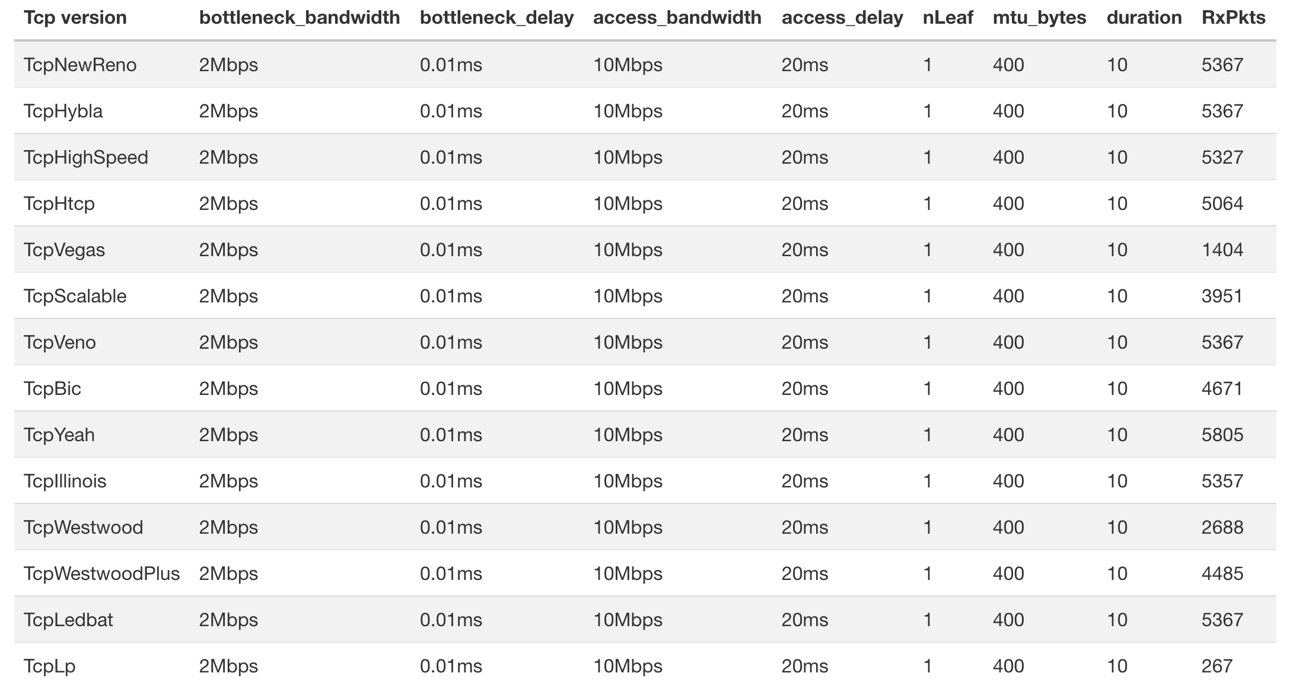
\includegraphics[width=0.8\linewidth]{figure/figure1.png}
	\caption{传统方法数据接收对比图}
	\label{figure1}
\end{figure}

由于要选择一个数据包接收效果尽可能好的协议,同时仿真智能体应基于时间,我们选择了TcpNewReno作为参照的仿真协议。通过这个协议可以得到传统方法的CWND图。

\begin{figure}[h]
	\centering
	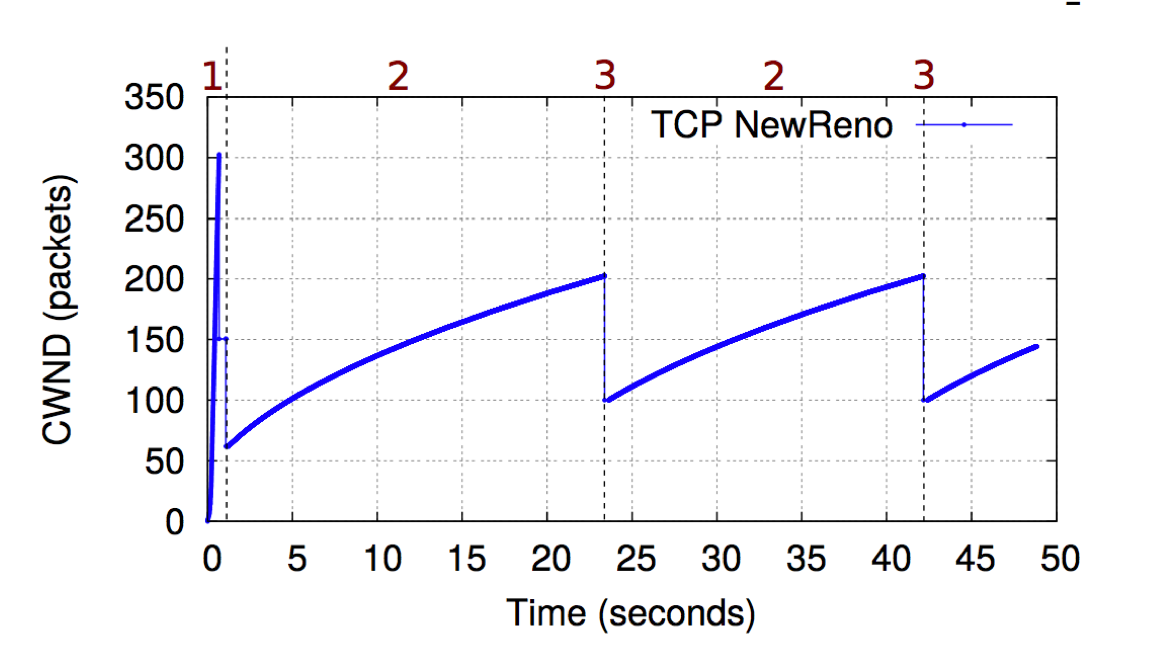
\includegraphics[width=0.6\linewidth]{figure/figure2.png}
	\caption{传统方法CWND曲线图}
	\label{figure2}
\end{figure}

对应着强化学习的方法,可以从QTCP论文之中获取吞吐量以及RTT的示意图。
接下来第一步,我们小组尝试改进论文中的DEMO,也就是自适应视频流传输的算法,尝试加快模型的收敛速度。
第二步,尝试传统方法从C++到Python的移植。
第三步,采用Deep Q-Learning算法进行训练,算法模型如下图。
第四步,改进reward和action。

\begin{figure}[htbp]
\centering
\begin{minipage}[t]{0.48\textwidth}
\centering
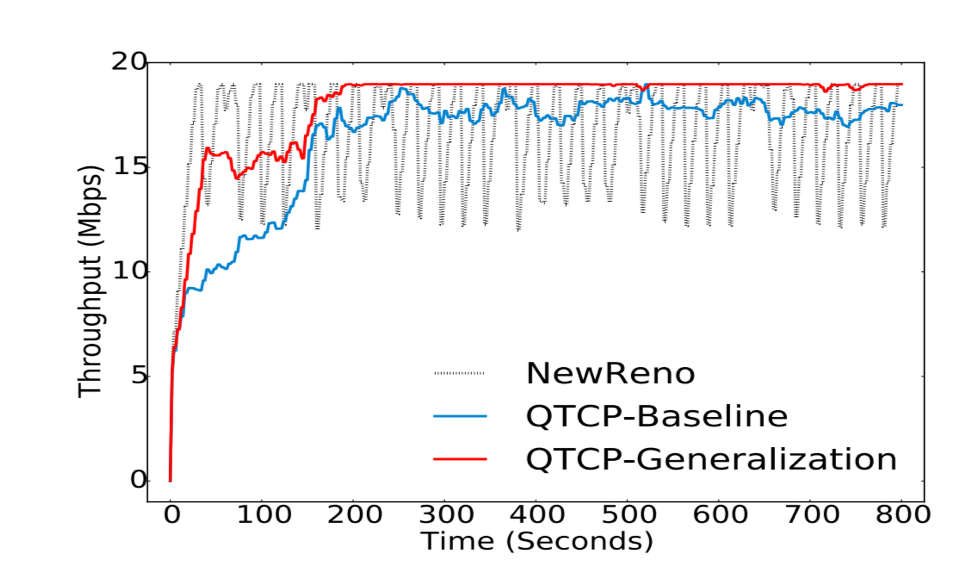
\includegraphics[width=6cm]{figure/figure3.png}
\caption{吞吐量}
\end{minipage}
\begin{minipage}[t]{0.48\textwidth}
\centering
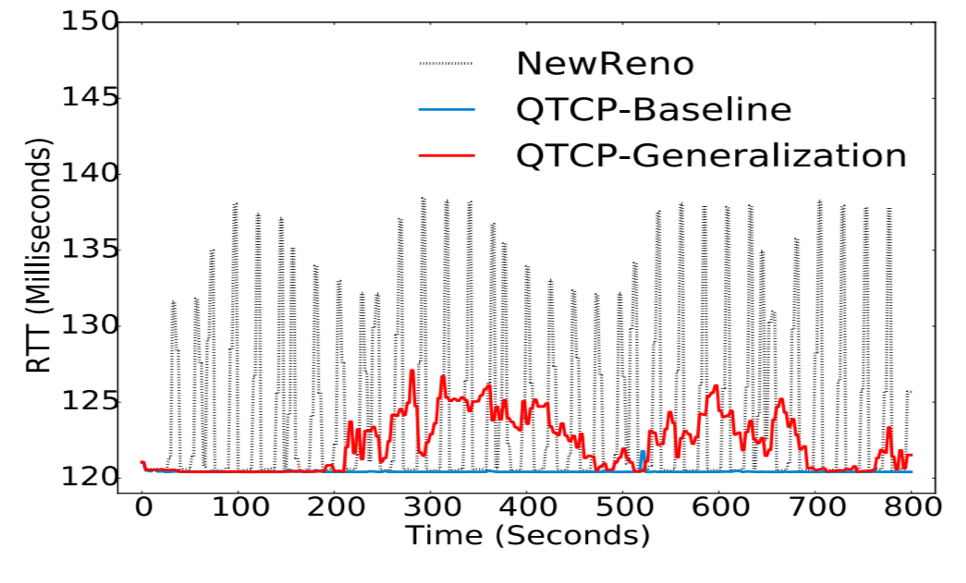
\includegraphics[width=6cm]{figure/figure4.png}
\caption{RTT}
\end{minipage}
\centering
	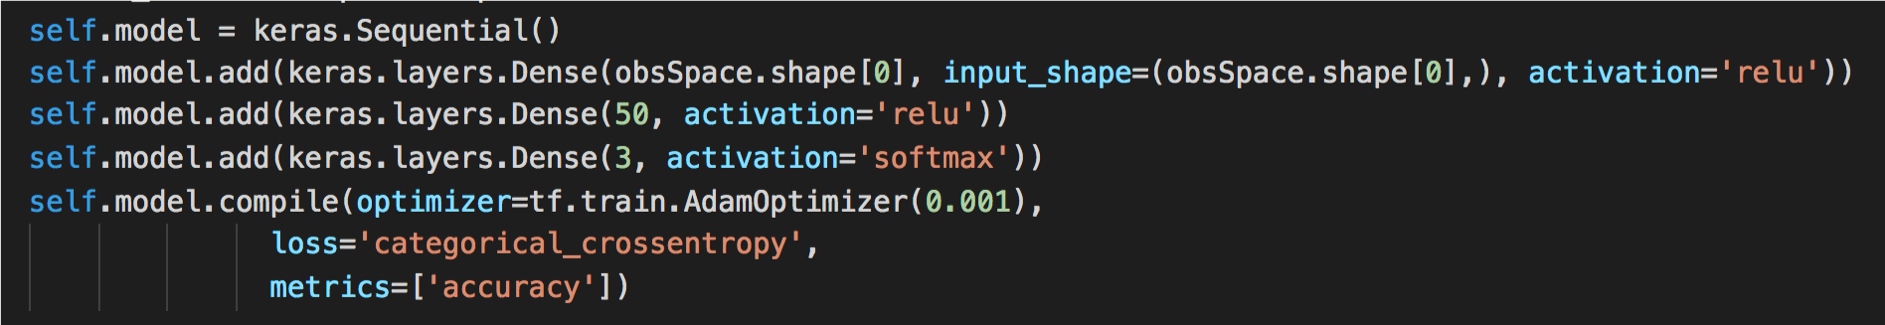
\includegraphics[width=0.8\linewidth]{figure/figure5.png}
	\caption{强化学习模型}
	\label{figure5}
\end{figure}

\section{评测结果}

\subsection{程序清单}

\begin{enumerate}
\item sim.cc:传统方法仿真脚本
\item tcp\_base.py:Deep Q-learning算法模型
\item tcp\_newreno.py:newreno算法实现
\item tcp-rl-env.cc:网络环境在强化学习当中的环境构建
\item tcp-rl.cc:强化学习环境构建
\item test\_tcp.py:强化学习运行脚本
\end{enumerate}

\subsection{实验结果}

\begin{figure}[htbp]
	\centering
	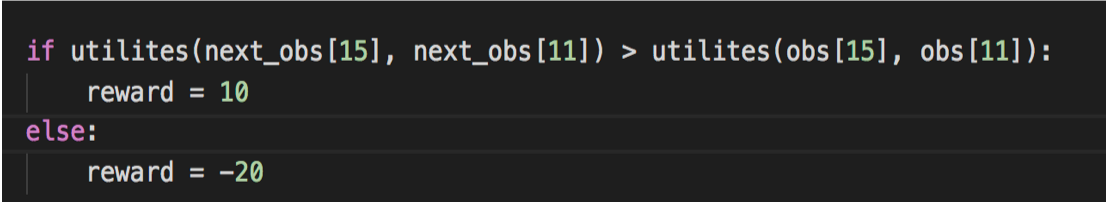
\includegraphics[width=0.8\linewidth]{figure/figure7.png}
	\caption{改进reward}
	\label{figure7}
	\centering
	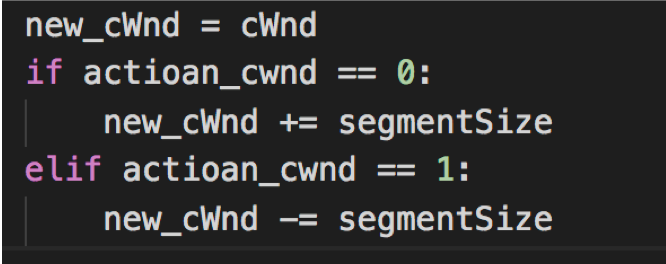
\includegraphics[width=0.6\linewidth]{figure/figure8.png}
	\caption{改进action}
	\label{figure8}
\end{figure}

\begin{figure}[htbp]
\centering
\begin{minipage}[t]{0.48\textwidth}
\centering
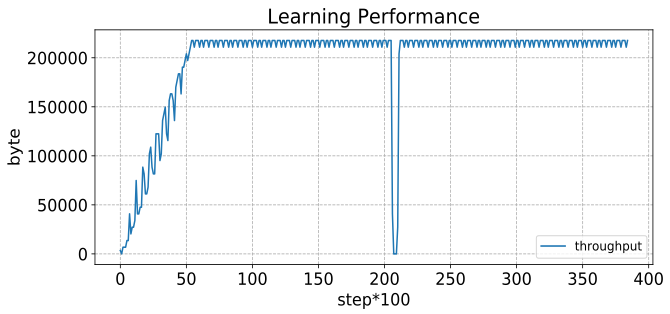
\includegraphics[width=6cm]{figure/figure9.png}
\caption{throughput}
\end{minipage}
\begin{minipage}[t]{0.48\textwidth}
\centering
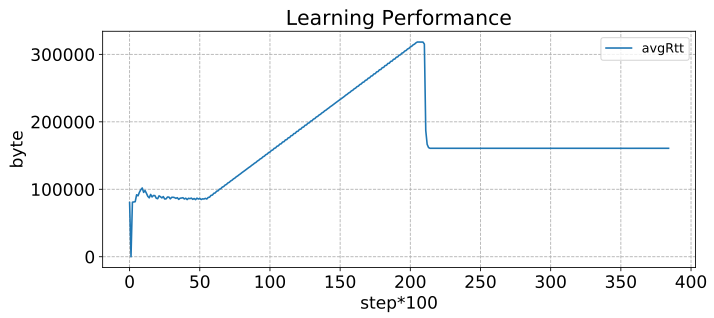
\includegraphics[width=6cm]{figure/figure10.png}
\caption{avgRTT}
\end{minipage}
\centering
\begin{minipage}[t]{0.48\textwidth}
\centering
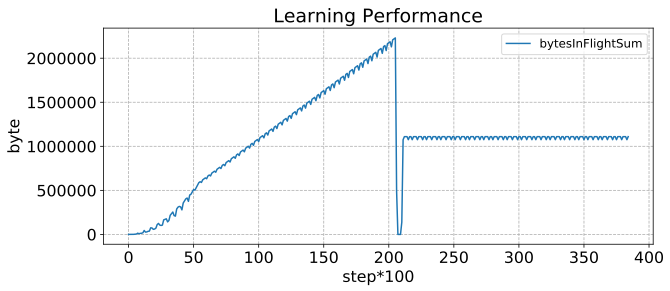
\includegraphics[width=6cm]{figure/figure11.png}
\caption{bytesInFlightSum}
\end{minipage}
\begin{minipage}[t]{0.48\textwidth}
\centering
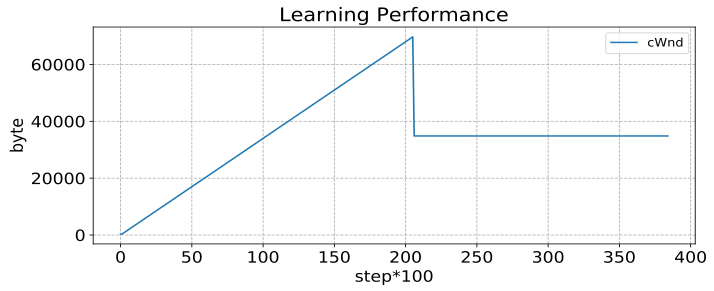
\includegraphics[width=6cm]{figure/figure12.png}
\caption{CWND}
\end{minipage}
\end{figure}

改进后,1个step的平均运行速度为0.007s,收敛速度也超过了论文水平。由此可见,强化学习方法在计算机网络领域作用是能起到作用的。

\section{讨论}

\subsection{问题讨论}

\begin{enumerate}
\item NS3的使用不熟悉,导致不知道该如何搭建相应的环境,花了很长的时间查看别人的代码,最终解决问题。
\item 强化学习的内容不清楚,在开始设计相关算法之前查阅相关资料。
\item 设计出来的action不合适,导致需要很多step才能看出相应的结果,这里通过调整action的步长快速看出效果,快速调节相关参数。
\item 基于事件的仿真智能体始终不能正常运行,后面改成基于时间的仿真智能体。
\end{enumerate}

\subsection{老师评论}

\subsection{反思与建议}

在课设的最开始,最好能先理顺整个文件目录的结构,以及整个项目的运行逻辑,比如使用传统方法还是强化学习方法,基于时间还是基于事件。这样能够比较有针对性的快速上手,从而节省时间。


\section{相关工作}

基于OpenAI有许多NS3仿真研究,主要包括:

\begin{enumerate}
\item TCP拥塞控制、自适应视频流传输等网络应用
\item OpenAI Gym扩展开发
\item 基于强化学习的网络问题解决方案
\end{enumerate}

我们的工作是在网络应用这一部分中实现了模型的优化,加快了模型的收敛速度与准确率。

\section{总结}

\subsection{完成工作}

钟嘉伦:
自适应视频流传输调研,模型移植调研,各种文档撰写。

孙昊海:
RL方法调研,强化学习模型搭建,强化学习模型调优。

\subsection{个人小结}

钟嘉伦:
这次的计算机网络课设对我还是有很大帮助的。首先是了解了计算机网络仿真的相关知识,比如学会了NS3仿真的基本操作以及计算机网络应用的系统结构。其次是了解了强化学习的基本过程,特别是强化学习在计算机网络领域的具体应用,从算法研究走向实际的工程之中。此外,课程答辩的准备以及文档方面的撰写也与以往不同,我写了两个版本的报告,由于对Latex不太熟练且图比较多,Latex版直到最后一刻还在调图片的显示。所以十分感谢有这样一次机会能让我发现自己的不足,从而提升自己。

孙昊海:
这次实验对我的启发非常大,之前一直是做的深度学习的内容,涉及到的领域都大多是自然语言处理以及图像处理等方面,这是我第一次接触强化学习的内容,强化学习在计算机网络上的应用也是非常的广。
ns3的使用之前也不太熟悉,有很多不懂的地方,花了非常多的时间去翻看别人的代码。tcp拥塞控制是一个很棒的选题,强化学习在这个应用上会发挥非常大的作用,在后续过程当中,我想把现有的模型继续调优,达到一个比较不错的效果。


\appendix

\section{附录}

参考文献如下:\cite{ns3-TCP-DoS-Attack,ns3-BLUE}。



\bibliographystyle{IEEEtran}
\bibliography{reference}

\end{document}
